\documentclass[10pt,a4paper]{article}
\usepackage[UTF8,fontset = windows]{ctex}
\setCJKmainfont[BoldFont=黑体,ItalicFont=楷体]{华文中宋}
\usepackage{amssymb,amsmath,amsfonts,amsthm,mathrsfs,dsfont,graphicx}
\usepackage{ifthen,indentfirst,enumerate,color,titletoc}
\usepackage{tikz}
\usepackage{makecell}
\usepackage{longtable}
%\usepackage{mathptmx}

\usetikzlibrary{arrows,calc,intersections,patterns,decorations.pathreplacing}
\usepackage[bf,small,indentafter,pagestyles]{titlesec}
\usepackage[top=1in, bottom=1in,left=0.8in,right=0.8in]{geometry}
\renewcommand{\baselinestretch}{1.65}
\newtheorem{defi}{定义~}
\newtheorem{eg}{例~}
\newtheorem{ex}{~}
\newtheorem{rem}{注~}
\newtheorem{thm}{定理~}
\newtheorem{coro}{推论~}
\newtheorem{axiom}{公理~}
\newtheorem{prop}{性质~}
\newcommand{\blank}[1]{\underline{\hbox to #1pt{}}}
\newcommand{\bracket}[1]{(\hbox to #1pt{})}
\newcommand{\onech}[4]{\par\begin{tabular}{p{.9\textwidth}}
A.~#1\\
B.~#2\\
C.~#3\\
D.~#4
\end{tabular}}
\newcommand{\twoch}[4]{\par\begin{tabular}{p{.46\textwidth}p{.46\textwidth}}
A.~#1& B.~#2\\
C.~#3& D.~#4
\end{tabular}}
\newcommand{\vartwoch}[4]{\par\begin{tabular}{p{.46\textwidth}p{.46\textwidth}}
(1)~#1& (2)~#2\\
(3)~#3& (4)~#4
\end{tabular}}
\newcommand{\fourch}[4]{\par\begin{tabular}{p{.23\textwidth}p{.23\textwidth}p{.23\textwidth}p{.23\textwidth}}
A.~#1 &B.~#2& C.~#3& D.~#4
\end{tabular}}
\newcommand{\varfourch}[4]{\par\begin{tabular}{p{.23\textwidth}p{.23\textwidth}p{.23\textwidth}p{.23\textwidth}}
(1)~#1 &(2)~#2& (3)~#3& (4)~#4
\end{tabular}}
\begin{document}
\begin{enumerate}[1.]

\item 用列举法表示下列集合:\\
(1) 十二生肖名称的集合;\\
(2) $10$以内的素数组成的集合;\\
(3) $\{y|y=x^2-1, \ -1<x<3, \ x\in \mathbf{Z}\}$.
\item 用描述法表示下列集合:\\
(1) 被$3$除余数等于1的整数的集合;\\
(2) 比$1$大又比$10$小的实数组成的集合;\\
(3) 平面直角坐标系内横轴上的点的坐标组成的集合.
\item 下面写法正确的是\bracket{20}.
\fourch{$0\in \{(0,1)\}$}{$1\in \{(0,1)\}$}{$(0,1)\in \{(0,1)\}$}{$(0,1)\in \{0,1\}$}
\item 集合$\{(x,y)|xy\ge 0, \ x\in \mathbf{R}, \ y\in \mathbf{R}\}$是指\bracket{20}.
\twoch{第一象限内的所有点}{第三象限内的所有点}{第一象限和第三象限内的所有点}{不在第二象限、第四象限内的所有点}
\item 用适当的方法表示下列集合:\\
(1) 方程$x^2-2=0$的实数解组成的集合;\\
(2) 两直线$y=2x+1$和$y=x-2$的交点组成的集合.
\item 已知集合$A=\{2,(a+1)^2,a^2+3a+3\}$, 且$1\in A$, 求实数$a$的值.
\item 指出下列各集合之间存在的关系:\\
(1) $A=\{x|x^2-2x+1=0\}$, $B=\{x|x^2-1=0\}$;\\
(2) $A=\{1,2,4,8\}$, $B=\{x|x\text{是}8\text{的正约数}\}$.
\item 下列写法正确的是\bracket{20}.
\fourch{$\varnothing \subsetneqq \{0\}$}{$0\subsetneqq \varnothing$}{$\varnothing \in \{0\}$}{$0\in \varnothing$}
\item 若集合$A=\{x|x=2n+1, \ n\in \mathbf{Z}\}$, 集合$B=\{x|x=4n-1, \ n\in \mathbf{Z}\}$, 则$A$、$B$的关系是\bracket{20}.
\fourch{$A\subseteq B$}{$A=B$}{$A\subsetneqq B$}{$B\subsetneqq A$}
\item 已知集合$A=\{1\}$, 集合$B=\{x|x^2-3x+a=0\}$, 且$A\subsetneqq B$, 求实数$a$的值.
\item 已知集合$A=\{x,y\}$, 集合$B=\{2x,2x^2\}$, 且$A=B$, 求集合$A$.
\item 已知集合$S=\{1,2\}$, 集合$T=\{x|ax^2-3x+2=0\}$, 且$S=T$, 求实数$a$的值.
\item 已知$a$是常数, 集合$M=\{x|x^2+x-6=0\}$, 集合$N=\{y|ay+2=0\}$, 且$N\subseteq M$, 求实数$a$的值.
\item 已知所有菱形组成的集合为$A$, 所有矩形组成的集合为$B$, 求$A\cap B$.
\item 已知集合$A=\{x|x\le 7\}$, 集合$B=\{x|x<2\}$, 集合$C=\{x|x>5\}$, 求$A\cap B$, $A\cap C$, $A\cap (B\cap C)$.
\item 已知集合$A=\{(x,y)|u=-x+1\}$, 集合$B=\{(x,y)|y=x^2-1\}$, 求$A\cap B$.
\item 已知集合$A=\{x|x\text{是锐角三角形}\}$, 集合$B=\{x|x\text{是钝角三角形}\}$, 求$A\cap B$, $A\cup B$.
\item 已知集合$A=\{x|x^2+px+15=0\}$, 集合$B=\{x|x^2-5x+q=0\}$, 且$A\cap B=\{3\}$, 求$p$、$q$的值和$A\cup B$.
\item 已知集合$A=\{x|x\le 1\}$, 集合 $B=\{x|x\ge a\}$, 且$A\cup B=\mathbf{R}$, 求$a$的取值范围.
\item 已知集合$A=\{x|x\text{是平行四边形}\}$, 集合$U=\{x|x\text{是至少有一组对边平行的四边形}\}$, 求$\complement _UA$.
\item 设$U=\mathbf{R}$, 集合$A=\{x|4-x>2x+1\}$, 求$\complement _UA$.
\item 已知集合$U=\{x|0<x\le 10, \ x\in \mathbf{N}\}$, 集合$A=\{1,2,4,5,9\}$, 集合$B=\{4,6,7,8,10\}$, 求$\complement _UA$, $\complement _UB$, $\complement _UA\cup \complement _UB$, $\complement _UA\cap \complement _UB$, $\complement _U(A\cap B)$, $\complement _U(A\cup B)$, 并指出其中相等的集合.
\item 用$A$、$B$的运算式表示图中的阴影部分:\\
(1) 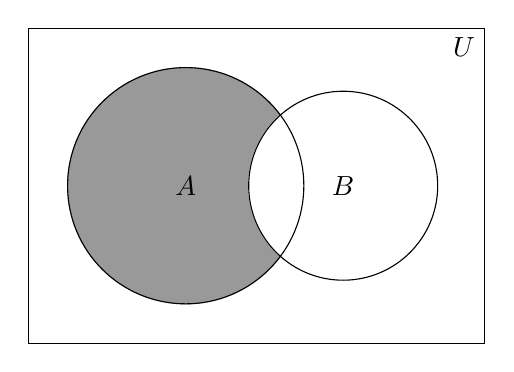
\begin{tikzpicture}
    \filldraw [gray!80] (0,0) circle (1.5);
    \filldraw [white] (2,0) circle (1.2);
    \draw (0,0) circle (1.5) node {$A$} (2,0) circle (1.2) node {$B$};
    \draw (-2,-2) rectangle (3.8,2) node [below left] {$U$};    
\end{tikzpicture} (2) 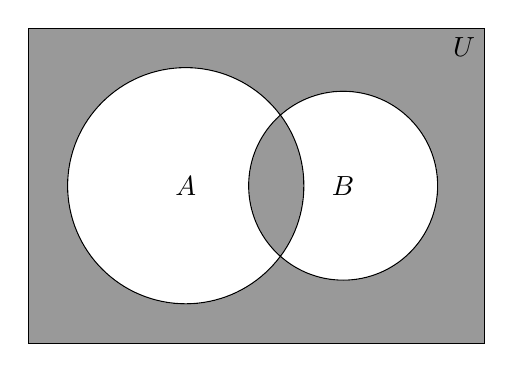
\begin{tikzpicture}
    \filldraw [gray!80] (-2,-2) rectangle (3.8,2);
    \filldraw [even odd rule, white] (0,0) circle (1.5) (2,0) circle (1.2);
    \draw (0,0) circle (1.5) node {$A$} (2,0) circle (1.2) node {$B$};
    \draw (-2,-2) rectangle (3.8,2) node [below left] {$U$};    
\end{tikzpicture}
\item 已知集合$A=\{1,4,x\}$, 集合$B=\{1,x^2\}$, 且$A\cup B=A$, 求$x$的值及集合$A$、$B$.
\item 已知集合$A=\{x|-2\le x\le 4\}$, 集合$B=\{x|-3<x<2\}$, 集合$C=\{x|-3\le x<0\}$, 求$A\cup B$, $(A\cap B)\cup C$, $(A\cup C)\cap (B\cup C)$.
\item 已知集合$U=\{x|x\ge 2\}$, 集合$A=\{y|3\le y<4\}$, 集合$B=\{z|2\le z<5\}$, 求$\complement _UA\cap B$, $\complement _UB\cup A$.
\item 已知集合$U=\{a,b,c,d,e,f\}$, 集合$A=\{a,b,c,d\}$, $A\cap B=\{a\}$, $\complement _U(A\cup B)=\{f\}$, 求集合$B$.
\item 判断下列语句是否为命题, 并在相应的括号内填入``是''或``否''.\\
(1) 正方形是四边形; \blank{20}\\
(2) $0$是自然数吗; \blank{20}\\
(3) 交集和并集; \blank{20}\\
(4) $3<\pi$. \blank{20}
\item 判断下列命题的真假, 并在相应的括号内填入``真命题''或``假命题''.\\
(1) 如果$a$、$b$都是奇数, 那么$a+b$是偶数; \blank{20}\\
(2) 一组对边平行且两对角线相等的四边形是平行四边形; \blank{20}\\
(3) 如果$|a|<2$, 那么$a<2$; \blank{20}\\
(4) 如果$A\cap B=A$, 那么$A\cup B=B$. \blank{20}
\item 如果$a$、$b$、$c$为实数, 设
$A:a=b=c=0$; $B:a,b,c$至少有一个为$0$; $C:a^2+\sqrt b+|c|=0$, 那么$A$\blank{20}$B$; $A$\blank{20}$C$; $B$\blank{20}$C$.(用符号``$\Rightarrow$''、``$\Leftarrow$''或``$\Leftrightarrow$''填空)
\item 已知命题$A$: 如果$x<3$, 那么$x<5$; 命题$B$: 如果$x\ge 3$, 那么$x\ge 5$; 命题$C$: 如果$x\ge 5$, 那么$x\ge 3$.填写各命题之间的关系:
$A$与$B$互为\blank{20}命题, $B$与$C$互为\blank{20}命题, $C$与$A$互为\blank{20}命题.
\item 写出命题``在$\triangle ABC$中, 如果$\angle C>\angle B$, 那么$AB>AC$''的逆命题、否命题和逆否命题, 并判断其真假.
\item 写出命题``如果$\alpha$, 那么$\beta$''的逆命题、否命题和逆否命题.
\item 写出命题``已知$a$、$b$、$c$是实数, 如果$ac<0$, 那么$ax^2+bx+c=0(a\ne 0)$有实数根''的逆命题.否命题和逆否命题, 并判断其真假.
\item 命题``若$x\ne 3$且$x\ne 4$, 则$x^2-7x+12\ne 0$''的逆否命题是\bracket{20}.
\twoch{若$x^2-7x+12=0$, 则$x=3$或$x=4$}{若$x^2-7x+12=0$, 则$x\ne 3$或$x\ne 4$}{若$x^2-7x+12\ne 0$, 则$x\ne 3$且$x\ne 4$}{若$x^2-7x+12=0$, 则$x=3$且$x=4$}
\item 如果命题$A$的逆命题是$B$, 命题$A$的否命题是$C$, 那么命题$B$是命题$C$的\bracket{20}.
\fourch{逆命题}{否命题}{逆否命题}{以上都不正确}
\item 试判断命题$A$: ``在$\triangle ABC$中, $BC^2=AC^2+AB^2$''与命题$B$: ``$\triangle ABC$是直角三角形''是否为等价命题, 并说明理由.
\item 试判断命题$A$: ``三角形任意两边之和大于第三边''与命题$B$: ``三角形任意两边之差小于第三边''是否为等价命题, 并说明理由.
\item 求证: 对角线不互相平分的四边形不是平行四边形.
\item 判断下列命题的真假, 并在相应的横线上填入``真命题''或``假命题''.\\
(1) 若$A\cap B\ne \varnothing$, $B\subsetneqq C$, 则$A\cap C\ne \varnothing$\blank{20};\\
(2) 方程$(a+1)x+b=0$($a$、$b\in \mathbf{R}$)的解为$x=-\dfrac b{a+1}$\blank{20};\\
(3)若命题$\alpha$、$\beta$、$\gamma$满足$\alpha \Rightarrow \beta$, $\beta \Rightarrow \gamma$, $\gamma \Rightarrow \alpha$, 则$\alpha \Leftrightarrow \gamma$\blank{20}.
\item 若$\alpha$: $\{2\}\subsetneqq B\subseteq \{2,3,4\}$, $\beta :B=\{2,4\}$, 则$\alpha$与$\beta$的推出关系是\bracket{20}.
\fourch{$\alpha \Rightarrow \beta$}{$\beta \Rightarrow \alpha$}{$\alpha \Leftrightarrow \beta$}{$\alpha \not\Rightarrow \beta$且$\beta \not\Rightarrow \alpha$}
(2)由命题甲成立, 可推出命题乙不成立, 下列说法一定正确的是\bracket{20}.
\twoch{命题甲不成立, 可推出命题乙成立}{命题甲不成立, 可推出命题乙不成立}{命题乙成立, 可推出命题甲成立}{命题乙成立, 可推出命题甲不成立}
\item 已知一个命题的否命题是``两组对边分别相等的四边形是平行四边形'', 试写出原命题的逆命题, 并判断原命题的真假.
\item 已知一个命题的逆命题是``若实数$a$、$b$满足$a=1$且$b=2$, 则$a+b<4$'', 试写出原命题的否命题, 并判断原命题的真假.
\item 类比$A\subseteq B\Leftrightarrow A\cap B=A$, 试再写出两个等价命题:\\
$A\subseteq B\Leftrightarrow$\blank{50};\\
$A\subseteq B\Leftrightarrow$\blank{50}.
\item 下列各题中命题$P$是命题$Q$的什么条件?\\
(1) $P$: 四边形的四条边相等, $Q$: 四边形是正方形;\\
(2) $P$: $\triangle ABC\cong \triangle DEF$,	$Q$: $\triangle ABC$的面积$=\triangle DEF$的面积;\\
(3) $P$: $x$是2的倍数, $Q$: $x$是6的倍数;\\
(4) $P$: 两个三角形全等, $Q$: 两个三角形的两角和一边对应相等.
\item 若$x$、$y$都是实数, 则``$xy=0$''是``$x=0$''的\blank{50}条件.
\item 若$x$、$y$、$z$都是实数, 则``$x\cdot y=y\cdot z$''是``$x=z$''的\blank{50}条件.
\item 若$x$、$y$、$z$都是实数, 则``$\dfrac xy=\dfrac yz$''是``$xz=y^2$''的\blank{50}条件.
\item 若$x$、$y$都是实数, 则``$|x|>|y|$''是``$x>y>0$''的\blank{50}条件.
\item 已知$l$、$m$、$n$都是自然数, ``$l+m+n$为偶数''是``$l$、$m$、$n$都是偶数''的什么条件? 为什么?
\item 有下列四组命题:
\textcircled{1} $P$: 集合$A\subseteq B$, $B\subseteq C$, $C\subseteq A$, 		$Q$: 集合$A=B=C$;
\textcircled{2} $P$: $A\cap B=A\cap C$, 					$Q$: $B=C$;
\textcircled{3} $P$: $(x-2)(x-3)=0$, 				$Q$: $\dfrac{x-2}{x-3}=0$;
\textcircled{4} $P$: 抛物线$y=ax^2+bx+c(a\ne 0)$过原点, $Q$: $c=0$.
其中$P$是$Q$的充要条件的有\bracket{20}.
\fourch{\textcircled{1} 、\textcircled{2} }{\textcircled{1} 、\textcircled{4} }{\textcircled{2} 、\textcircled{3} }{\textcircled{2} 、\textcircled{4}}
\item 写出使实数$a$、$b$一正一负的充要条件.
\item 求证: 实数$a$、$b$均大于0的充要条件是$\begin{cases} a+b>0, \\ ab>0. \end{cases}$
\item 命题``$x\in M$或$x\in P$''是命题``$x\in M\cap P$''的什么条件?
\item 写出命题``$x>3$''的一个充分条件和一个必要条件.
\item 如果$\alpha$是$\beta$的充分非必要条件, 那么$\overline{\alpha }$是$\overline{\beta }$的什么条件?
\item 如果$A$是$B$的必要条件, $C$是$B$的充分条件, $A$是$C$的充分条件, 那么$B$、$C$分别是$A$的什么条件?
\item 填空:
已知集合$A=\{a|a$具有性质$p\}$, $B=\{b|b$具有性质$q\}$.\\
(1) 若$A\subseteq B$, 则$p$是$q$的\blank{50}条件;\\
(2) 若$A\supseteq B$, 则$p$是$q$的\blank{50}条件;\\
(3) 若$A=B$, 则$p$是$q$的\blank{50}条件.
\item 试用子集与推出关系来判断命题$A$是命题$B$的什么条件.\\
(1) $A$: 该平面图形是四边形, $B$: 该平面图形是梯形;\\
(2) $A$: $x=2$, $B$: $(x-5)(x-2)=0$;\\
(3) $A$: $x^2=y^2$, $B$: $x=y$;\\
(4) $A$: $a=2$, $B$: $a\le 2$.
\item 如果命题$p$: $m<-3$, 命题$q$: 方程$x^2-x-m=0$无实数根, 那么$p$是$q$的什么条件?
\item 已知命题$\alpha$: $2\le x<4$, 命题$\beta$: $3m-1\le x\le -m$, 且$\alpha$是$\beta$的充分条件, 求实数$m$的取值范围.
\item 如果命题$p$: $A\subseteq B$, 命题$q$: $A\subsetneqq B$, 那么$p$是$q$的什么条件?
\item 已知$a$为实数, 写出关于$x$的方程$ax^2+2x+1=0$至少有一个实数根的一个充要条件、一个充分条件、一个必要条件.
\item 下列命题中正确的是\bracket{20}.
\twoch{自然数集$\mathbf{N}$中最小的数是$1$}{空集是任何集合的真子集}{如果$A\subseteq B$, 且$A\ne B$, 那么$A$是$B$的真子集}{$\{y|y=x+3,\ x\in \mathbf{N}\}$中的最小值是4}
\item 若$A\cap B=A$, 则\bracket{20}.
\fourch{$\complement _BA\cup A=\varnothing$}{$\complement _BA\cap A=\varnothing$}{$\complement _BA\cup \complement _BB=\varnothing$}{$\complement _BA\cap A=\varnothing$}
\item 已知$I$是全集.若$M$、$P$、$S$是$I$的3个子集, 则图中阴影部分所表示的集合是\bracket{20}.
\begin{center}
    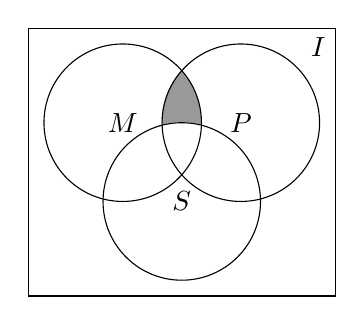
\begin{tikzpicture}
        \begin{scope}
            \clip (0,0) circle (1);
            \filldraw [gray!80] (1.5,0) circle (1);
        \end{scope}
        \filldraw [white] (0.75,-1) circle (1);
        \draw (0,0) circle (1) node {$M$};
        \draw (1.5,0) circle (1) node {$P$};
        \draw (0.75,-1) circle (1) node {$S$};
        \draw (-1.2,-2.2) rectangle (2.7,1.2) node [below left] {$I$};
    \end{tikzpicture}
\end{center}
\fourch{$(M\cap P)\cap S$}{$(M\cap P)\cup S$}{$(M\cap P)\cap \complement _IS$}{$(M\cap P)\cup \complement _IS$}
\item 若命题$p$: $x^2-5x+6=0$, 命题$q$: $x=2$, 则$p$是$q$的\blank{50}条件。
\item 若$p$: 四边形是正方形, $q$: 四边形的两条对角线互相垂直平分, 则$p$是$q$的\blank{50}条件.
\item 若$p$: 抛物线$y=ax^2+bx+c$过原点, $q$: $c=0$, 则$p$是$q$的\blank{50}条件.
\item 若$p$: $a>b$, $q$: $a^2>b^2$, 则$p$是$q$的\blank{50}条件.
\item 若方程$x^2+px+4=0$的解集为$A$, 方程$x^2+x+q=0$的解集为$B$, 且$A\cap B=\{4\}$, 则集合$A\cup B$的所有子集是\blank{50}.
\item 对上海市某校学生进行调查, 结果如下: 成语同典拥有率为$84\%$, 古汉语词典拥有率为$78\%$.同时拥有上述两种词典的学生占全校学生的$66\%$, 求上述两种词典都没有的学生所占的比例.
\item 已知集合$A=\{x|-2<x\le 1\}$, 集合$B=\{x|x\ge 1x<-2\}$, 求$A\cup B$, $A\cap B$.
\item 已知集合$A=\{x|-1<x<1$或$x\ge 3\}$, 集合$U=\{x|x\ge 2x<1\}$, 求$\complement _UA$.
\item 写出命题: 若$x>1$, 则$x>0$的逆命题、否命题、逆否命题, 并指出哪些是真命题.
\item 已知集合$A=\{x|x^2+px+q=0\}$, 集合$B=\{x|x^2-x+r=0\}$, 且$A\cap B=\{-1\}$, $A\cup B=\{-1,2\}$, 求$p$、$q$、$r$的值.
\item 已知全集$U=\mathbf{R}$, 集合$A=\{x|x\le a-1\}$, 集合$B=\{x|x>a+2\}$, 集合$C=\{x|x<0$或$x\ge 4\}$.若$\complement _U(A\cup B)\subseteq C$, 求实数$a$的取值范围.
\item 若集合$M=\{a|a=x+\sqrt 2y,\ x,y\in \mathbf{Q}\}$, 则下列结论正确的是\bracket{20}.
\fourch{$M\subseteq \mathbf{Q}$}{$M=\mathbf{Q}$}{$M\supsetneqq \mathbf{Q}$}{$M\subsetneqq \mathbf{Q}$}
\item 若$A$是$B$的必要非充分条件, $B$是$C$的充要条件, $C$是$D$的必要非充分条件, 则$D$是$A$的\blank{50}条件, $C$是$A$的\blank{50}条件.
\item 已知全集$U=\{x|x$为不大于$20$的素数$\}$.若$A\cap \complement _UB=\{3,5\}$, $\complement _UA\cap B=\{7,19\}$, $\complement _U(A\cup B)=\{2,17\}$, 则$A=$\blank{50}, $B=$\blank{50}.
\item 已知集合$P=\{x|-2\le x\le 5\}$, 集合$Q=\{x|k+1\le x\le 2k-1\}$, 且$Q\subseteq P$, 求实数$k$的取值范围.
\item 已知集合$A=\{x|(a-1)x^2+3x-2=0\}$, 是否存在这样的实数$a$, 使得集合$A$有且仅有两个子集? 若存在, 求出实数$a$的值及对应的两个子集;若不存在.请说明理由.
\item 解不等式: $2(x+1)-3(x-2)>8$.
\item 解不等式组: $\begin{cases} 3x-2(5-3x)>8, \\ 2x\le 2(2x+3). \end{cases}$
\item 判断下列语句是否正确, 并在相应的横线内填入``$\checkmark$''或``$\times$''.\\
(1) 若$ax>b$, 则$x>\dfrac ba(a\ne 0)$.\blank{20};\\
(2) 若$a^2x>a^2y$, 则$x>y$.\blank{20};\\
(3) 若$a>b>0$, $c>d>0$, 则$\dfrac ac>\dfrac bd$.\blank{20};\\
(4) 若$a>b$, 则$a^2>ab$.\blank{20}.
\item 如果$a^2>b^2$, 那么下列不等式中正确的是\bracket{20}.
\fourch{$a>0>b$}{$a>b>0$}{$|a|>|b|$}{$a>|b|$}
\item 如果$a<b<0$, 那么下列不等式中正确的是\bracket{20}.
\fourch{$\dfrac{-a}{-b}<1$}{$a^2>ab$}{$\dfrac 1{b^2}<\dfrac 1{a^2}$}{$\dfrac 1a<\dfrac 1b$}
\item 如果$a<0<b$, 那么下列不等式中正确的是\bracket{20}.
\fourch{$\sqrt {-a}<\sqrt b$}{$a^2<b^2$}{$a^3<b^3$}{$ab>b^2$}
\item 证明: 如果$a>b$, $c<0$, 那么$(a-b)c<0$.
\item 证明: 如果$a<b<0$, 那么$0>\dfrac 1a>\dfrac 1b$.
\item 用``$>$''或``$<$''号填空: 如果$a<b<0$, 那么\\
(1) $\sqrt [n]{-a}$\blank{50}$\sqrt [n]{-b}(n\ge 2,n\in \mathbf{N}^*)$;\\
(2) $\dfrac 1{a^{2n}}$\blank{50}$\dfrac 1{b^{2n}}(n\in \mathbf{N}^*)$.
\item 比较$x(x-y)$与$y(x-y)(x\ne y)$的大小.
\item 比较$(3a+1)(a+1)$与$2(a+1)^2-3$的大小.
\item 比较$(t+1)(t-5)$与$(t-2)^2$的大小.
\item 已知$a>2$, 解关于$x$的方程$ax+4<2x+a^2$.
\item 已知$m<1$, 解关于$x$的方程$mx+1<x+m^3$.
\item 已知$p\ne q$, 解关于$x$的方程$(p-q)x<p^2-q^2$.
\item 解关于$x$的方程$mx+4<m^2+2x$.
\item 甲乙两个工厂今年的产值分别为$25000$万元、$20000$万元.如果甲工厂每年增加产值$500$万元, 乙工厂每年增加产值$1000$万元, 那么几年后乙工厂的产值超过甲工厂的产值?
\item 如果$a>b$, 那么$\dfrac 1a<\dfrac 1b$成立的充要条件是\blank{50}.
\item 解关于$x$的不等式: $a^2(x-1)>b^2(1+x)+2ab$, 其中$a$、$b\in \mathbf{R}^+$.
\item 已知$x$、$y\in \mathbf{R}$, 比较$x^2+y^2$与$2(2x-y)-5$的大小.
\item 解不等式: $2x^2-3x+1<0$.
\item 解不等式: $(x+1)^2-6>0$.
\item 解不等式: $x(x-1)<x(2x-3)+1$.
\item 解不等式: $-x^2+2x+35>0$.
\item 解不等式: $(x-2)(3-x)\le 0$.
\item 解不等式: $2x-1\ge x^2$.
\item 解关于$x$的不等式: $(x-a)(x-1)<0(a>1)$.
\item 解关于$x$的不等式: $(x-a)(x-2a)<0(a>0)$.
\item 写出一个解集只含一个元素的一元二次不等式.
\item 解不等式组: $\begin{cases} 6-x-x^2\le 0, \\ x^2+3x-4<0. \end{cases}$.
\item 解不等式组: $\begin{cases} 4x^2-27x+18>0, \\ x^2-6x+4<0. \end{cases}$.
\item 已知集合$U=\mathbf{R}$, 且集合$A=\{x|x^2-16<0\}$, 集合$B=\{x|x^2-4x+3\ge 0\}$, 求:\\
(1) $A\cap B$;\\
(2) $A\cup B$;\\
(3) $\complement _U(A\cap B)$;\\
(4) $\complement _UA\cup \complement _UB$.
\item 已知不等式$x^2+ax+b<0$的解集为$(-3,-1)$, 求实数$a$、$b$的值.
\item 已知关于$x$的二次方程$2x^2+ax+1=0$无实数解, 求实数$a$的取值范围.
\item 已知$P(a,b)$为正比例函数$y=2x$的图像上的点, 且$P$与$B(2,-1)$之间的距离不超过$3$, 求$a$的取值范围.
\item 某船从甲码头沿河顺流航行$75$千米到达乙码头, 停留$30$分钟后再逆流航行$126$千米到达丙码头.如果水流的速度为每小时$4$千米, 该船要在$5$小时内完成航行任务, 那么船的速度每小时至少为多少千米?
\item 解不等式组: $\begin{cases} 3x^2+x-2\ge 0, \\ 4x^2-15x+9>0. \end{cases}$
\item 已知关于$x$的不等式组$\begin{cases} (2x-3)(3x+2)\le 0, \\ x-a>0 \end{cases}$无实数解, 求实数$a$的取值范围.
\item 当$k$取何值时, 关于$x$的不等式$2kx^2+kx-\dfrac 38<0$对于一切实数$x$都成立?
\item 已知关于$x$的不等式$ax^2+bx+c>0$的解集是$\{x|x>2$或$x<\dfrac 12\}$, 求关于$x$的不等式$ax^2-bx+c\le 0$的解集.
\item 某商品每件成本为$80$元, 售价为$100$元, 每天售出$100$件.若售价降低$x$成($1$成即$10\%$), 售出商品的数量就增加$\dfrac 85x$成.若要求该商品一天的营业额至少为$10260$元, 且又不能亏本, 求$x$的取值范围.
\item 解不等式: $\dfrac 1x<1$.
\item 解不等式: $\dfrac{4x+3}{x-1}>5$.
\item 解不等式: $\dfrac 2x<\dfrac 2{x-3}$.
\item 解不等式: $\dfrac 1{x-4}\le 1-\dfrac x{4-x}$.
\item 求当$k$为何值时, 关于$x$的方程$\dfrac{4k-3x}{k+2}=2x$的解分别是:\\
(1) 正数;\\
(2) 负数.
\item 解不等式: $|x^2-3|<2$.
\item 解不等式: $|\dfrac 1{2-x}|\ge 2$.
\item 解不等式: $|x^2-3x+2|\le 0$.
\item 解不等式: $|\dfrac x{x+1}|>\dfrac x{x+1}$.
\item 解不等式: $|x-3|<x-1$.
\item 若$a<b<0$, 则不等式$\dfrac{x+a}{x+b}>0$的解集是\blank{50}.
\item 解不等式: $4\le|x^2-4x|<5$.
\item 解不等式: $\dfrac 1{|x|}>x$.
\item 已知不等式$|ax+1|\le b$的解集是$[-1,3]$, 求$a$、$b$的值.
\item 如果$a$、$b\in \mathbf{R}$, 且$ab>0$, 那么下列不等式中正确的是\bracket{20}.
\fourch{$a^2+b^2>2ab$}{$a+b\ge 2\sqrt {ab}$}{$\dfrac 1a+\dfrac 1b>\dfrac 2{\sqrt {ab}}$}{$\dfrac ba+\dfrac ab\ge 2$}
\item 设$ab\ne 0$, 利用基本不等式有如下证明: $\dfrac ba+\dfrac ab=\dfrac{{b^2}+{a^2}}{ab}\ge \dfrac{2ab}{ab}=2$. 试判断这个证明过程是否正确. 若正确, 请说明每一步的依据; 若不正确, 请说明理由.
\item 已知$a$、$b\in \mathbf{R}$, 比较$|a|+\dfrac{|b|}2$与$\sqrt 2\cdot \sqrt {|ab|}$的大小.
\item 已知$0<x<\dfrac 12$, 求当$x$取何值时, $x(1-2x)$的值最大.
\item 已知$a>0$, 求证: $a+a^3\ge 2a^2$.
\item 用一根长为$l$的铁丝制成一个矩形框架.当长、宽分别为多少时, 框架的面积最大?
\item 已知$x$、$y\in \mathbf{R}^+$, 且$x+y=1$, 求当$x$、$y$分别取何值时, $\dfrac 1x+\dfrac 1y$的值最小.
\item 已知$x>-1$, 求当$x$取何值时, $x+\dfrac 4{x+1}$的值最小.
\item 已知$a+b=1$, 求证: $a^2+b^2\ge \dfrac 12$.
\item 建造一个容积为$8$立方米、深为$2$米的长方形无盖水池.如果池底和池壁的造价每平方米分别为$120$元和$80$元, 那么水池的最低造价是多少元?
\item 求证: $(ac+bd)^2\le (a^2+b^2)(c^2+d^2)$.
\item 已知$x>y$, 求证: $x^3-y^3>x^2y-xy^2$.
\item 已知实数$a\ge 3$, 求证: $\sqrt a-\sqrt {a-1}<\sqrt {a-2}-\sqrt {a-3}$.
\item 已知$a$、$b$、$c$是不全相等的整数, 求证: $(a^2+1)(b^2+1)(c^2+1)>8abc$.
\item 设$a$、$b$、$c\in \mathbf{R}^+$, 求证: $\dfrac{b+c}a+\dfrac{c+a}b+\dfrac{a+b}c\ge 6$.
\item 已知$a>0$, $b>0$, 求证: $\dfrac a{\sqrt b}+\dfrac b{\sqrt a}\ge \sqrt a+\sqrt b$.
\item 求证: $|\dfrac{a^2-1}{a^2+1}|\le 1$.
\item 如果$a\in \mathbf{R}$, 且$a^2+a<0$, 那么$a$、$a^2$、$-a$、$-a^2$的大小关系是\bracket{20}.
\fourch{$-a<-a^2<a<a^2$}{$a<-a^2<a^2<-a$}{$-a^2<a<a^2<-a$}{$-a^2<a<-a<a^2$}
\item 不等式$\dfrac{x^2}{x-1}\ge 0$的解是\bracket{20}.
\fourch{$(1,+\infty)$}{$[1+\infty)$}{$(1,+\infty)\cup \{0\}$}{$[1,+\infty)\cup \{0\}$}
\item 不等式$1+|x+1|<0$的解集是\bracket{20}.
\fourch{$(-\infty ,-2)$}{$(-2,0)$}{$\mathbf{R}$}{$\varnothing$}
\item 证明: 如果$a>b>0$, $c>d>0$, 那么$a^2c>b^2d$.
\item 证明: $a^2+b^2+2\ge 2(a+b)$.
\item 证明: 如果$a$、$b$、$c$都是正数, 那么$(a+b)(b+c)(c+a)\ge 8abc$.
\item 解不等式: $2(x+1)(x+2)>(x+3)(x+4)$.
\item 解不等式: $-3x^25x-4<0$.
\item 解不等式: $4x^2-20x+25\le 0$.
\item 解不等式: $x^2-16x+64>0$.
\item 解不等式组: $\begin{cases} x^2-16<0, \\ x^2-4x+3\ge 0. \end{cases}$.
\item 解不等式组: $4<x^2-x-2<10$.
\item 解不等式: $|\dfrac{3x-9}2|\le 6$.
\item 解不等式: $3<|x-2|<5$.
\item 解不等式: $|\dfrac 1x|<\dfrac 45$.
\item 下列四对不等式(组)中, 哪几对具有相同的解集?\\
(1) $-\dfrac 12x^2+3x+\dfrac{27}2>0$与$x^2-6x-27>0$;\\
(2) $4<x^2-x+2<10$与$\begin{cases} x^2-x+2<10, \\ x^2-x+2>4; \end{cases}$\\
(3) $|2x+1|<5$与$2x+1<5$或$2x+1>-5$;\\
(4) $\dfrac{x-1}{x+1}<2$与$x-1<2(x+1)$.
\item 已知关于$x$的不等式$2x^2-2(a-1)x+(a+3)>0$的解集是$\mathbf{R}$, 求实数$a$的取值范围.
\item 已知函数$y=(m-1)x^2+(m-3)x+(m-1)$, $m$取什么实数时, 函数图像与$x$轴\\
(1) 没有公共点?\\
(2) 只有一个公共点?\\
(3) 有两个不同的公共点?
\item 当$k$是什么实数时, 关于$x$的方程$2x+k(x+3)=4$的解是正数?
\item 已知直角三角形的周长为$4$, 求这个直角三角形面积的最大值, 并求此时各边的长.
\item 求证: $(\dfrac{a+b}2)^2\le \dfrac{a^2+b^2}2$.
\item 求不等式$5\le x^2-2x+2<26$的正整数解.
\item 已知$x$、$y\in [a,b]$.\\
(1) 求$x+y$的范围;\\
(2) 若$x<y$, 求$x-y$的范围.
\item 当$k$为什么实数时, 方程组$\begin{cases} 3x-6y=1, \\ 5x-ky=2 \end{cases}$的解满足$x<0$且$y<0$的条件?
\item 当$k$为什么实数时, 方程组$\begin{cases} 4x+3y=60, \\ kx+(k+2)y=60 \end{cases}$的解满足$x>y>0$的条件?
\item 已知$m<n$, 试写出一个形如$ax^2+bx+c>0$的一元二次不等式, 使它的解集分别为:\\
(1) $(-\infty ,m)\cup (n,+\infty)$;\\
(2) $(m,n)$.
\item 下列各图像中, 哪些是函数的图像, 哪些不是函数的图像? 为什么?
\begin{center}
    \begin{tikzpicture}[>=latex,scale = 0.9]
        \draw [->] (-2,0) -- (2,0) node [below] {$x$};
        \draw [->] (0,-2) -- (0,2) node [left] {$y$};
        \draw (0,0) node [below left] {$O$};
        \draw [domain = {-pi/2}:{pi/2}] plot ({\x},{-sin(2*\x/pi*180)});
        \draw (0,-2) node [below] {(1)};
    \end{tikzpicture}
    \begin{tikzpicture}[>=latex,scale = 0.9]
        \draw [->] (-2,0) -- (2,0) node [below] {$x$};
        \draw [->] (0,-2) -- (0,2) node [left] {$y$};
        \draw (0,0) node [below right] {$O$};
        \draw [domain = {-pi/2}:{pi/2}] plot ({sin(2*\x/pi*180)},{\x});
        \draw (0,-2) node [below] {(2)};        
    \end{tikzpicture}
    \begin{tikzpicture}[>=latex,scale = 0.6]
        \draw [->] (-1,0) -- (5,0) node [below] {$x$};
        \draw [->] (0,-1) -- (0,5) node [left] {$y$};
        \draw (0,0) node [below left] {$O$};
        \foreach \i in {0,1,2,3} 
        {   
            \draw (\i,{\i+1}) -- ({\i+1},{\i+1});
            \filldraw [fill = white, draw = black] (\i,{\i+1}) circle (0.05);
            \filldraw ({\i+1},{\i+1}) circle (0.05);
        };
        \filldraw [fill = white, draw = black] (0,0) circle (0.05);
        \foreach \i in {1,2,3,4}
        {
            \draw (\i,0.1) -- (\i,0) node [below] {$\i$};
            \draw (0.1,\i) -- (0,\i) node [left] {$\i$};
        };
        \draw (2,-1) node [below] {(3)};
    \end{tikzpicture}
    \begin{tikzpicture}[>=latex,scale = 0.6]
        \draw [->] (-1,0) -- (5,0) node [below] {$x$};
        \draw [->] (0,-1) -- (0,5) node [left] {$y$};
        \draw (0,0) node [below left] {$O$};
        \foreach \i in {0,1,2,3} 
        {   
            \draw ({\i+1},\i) -- ({\i+1},{\i+1});
            \filldraw [fill = white, draw = black] ({\i+1},{\i+1}) circle (0.05);
            \filldraw ({\i+1},\i) circle (0.05);
        };
        \filldraw [fill = white, draw = black] (0,0) circle (0.05);
        \foreach \i in {1,2,3,4}
        {
            \draw (\i,0.1) -- (\i,0) node [below] {$\i$};
            \draw (0.1,\i) -- (0,\i) node [left] {$\i$};
        };
        \draw (2,-1) node [below] {(4)};
    \end{tikzpicture}
\end{center}
\item 选择题:
下列各组函数$f(x)$与$g(x)$表示同一个函数的是\bracket{20}.
\onech{$f(x)=\dfrac{{x^2}-1}{x+1}$, $g(x)=x-1$}{$f(x)=|x|$, $g(x)=\begin{cases} x, & x\ge 0, \\ -x, & x<0 \end{cases}$}{$f(x)=x^0$, $g(x)=1$}{$f(x)=(\sqrt x)^2$, $g(x)=\sqrt {x^2}$}
\item 求函数$y=\dfrac 1{x^2+2x-3}$的定义域.
\item 求函数$y=\sqrt {4-3x-x^2}$的定义域.
\item 求函数$y=\sqrt {x-2}+\sqrt {x+3}$的定义域.
\item 求函数$y=\dfrac 1{x+2}+\dfrac 1{\sqrt {5-x}}$的定义域.
\item 若$f(x)=x^2+px+q$, 且$f(1)=0$, $f(2)=0$, 求$f(-1)$的值.
\item 观察下列各函数, 并写出他们的值域:
\begin{center}
    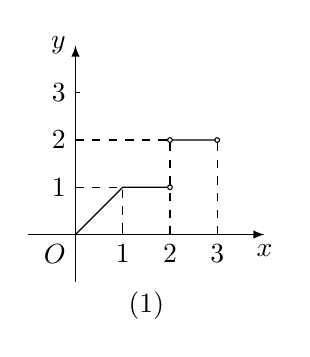
\begin{tikzpicture}[>=latex,scale = 0.6]
        \draw [->] (-1,0) -- (4,0) node [below] {$x$};
        \draw [->] (0,-1) -- (0,4) node [left] {$y$};
        \draw (0,0) node [below left] {$O$};
        \foreach \i in {1,2,3}
        {
          \draw (\i,0.1) -- (\i,0) node [below] {$\i$};
          \draw (0.1,\i) -- (0,\i) node [left] {$\i$};          
        };
        \draw (0,0) -- (1,1) -- (2,1) (2,2) -- (3,2);
        \draw [dashed] (0,1) -- (1,1) -- (1,0) (0,2) -- (2,2) (2,0) -- (2,2) (3,0) -- (3,2);
        \filldraw [fill = white, draw = black] (2,1) circle (0.05) (2,2) circle (0.05) (3,2) circle (0.05);
        \draw (1.5,-1) node [below] {(1)};
    \end{tikzpicture}
    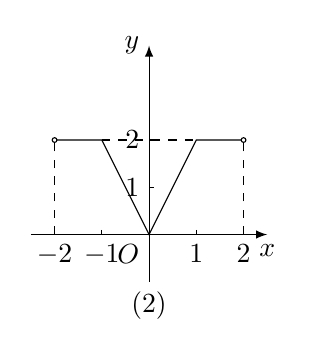
\begin{tikzpicture}[>=latex,scale = 0.6]
        \draw [->] (-2.5,0) -- (2.5,0) node [below] {$x$};
        \draw [->] (0,-1) -- (0,4) node [left] {$y$};
        \draw (0,0) node [below left] {$O$};
        \foreach \i in {1,2}
        {
          \draw (\i,0.1) -- (\i,0) node [below] {$\i$};
          \draw (0.1,\i) -- (0,\i) node [left] {$\i$};          
        };
        \foreach \i in {-1,-2}
        {
            \draw (\i,0.1) -- (\i,0) node [below] {$\i$};
        };
        \draw (-2,2) -- (-1,2) -- (0,0) -- (1,2) -- (2,2);
        \draw [dashed] (-2,0) -- (-2,2) (2,0) -- (2,2) (-1,2) -- (1,2);
        \filldraw [fill = white, draw = black] (-2,2) circle (0.05) (2,2) circle (0.05);
        \draw (0,-1) node [below] {(2)};
    \end{tikzpicture}
    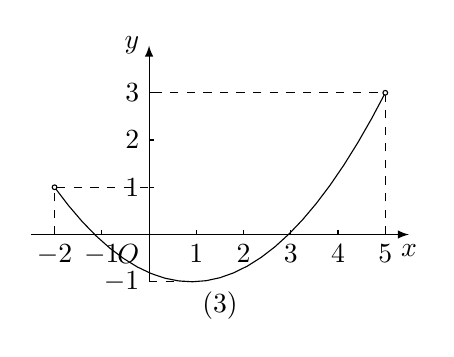
\begin{tikzpicture}[>=latex,scale = 0.6]
        \draw [->] (-2.5,0) -- (5.5,0) node [below] {$x$};
        \draw [->] (0,-1) -- (0,4) node [left] {$y$};
        \draw (0,0) node [below left] {$O$};
        \foreach \i in {-2,-1,1,2,3,4,5}
        {
            \draw (\i,0.1) -- (\i,0) node [below] {$\i$};
         
        };
        \foreach \i in {-1,1,2,3}
        {
            \draw (0.1,\i) -- (0,\i) node [left] {$\i$}; 
        };
        \draw [domain = -2:5] plot (\x,{2/49*(3+2*sqrt(2))*\x*\x+4/49*(-1-3*sqrt(2))*\x+(17-40*sqrt(2))/49});
        \draw [dashed] (0,-1) -- ({7*sqrt(2)-9},-1) (5,0) -- (5,3) -- (0,3) (-2,0) -- (-2,1) -- (0,1);
        \filldraw [fill = white, draw = black] (-2,1) circle (0.05) (5,3) circle (0.05);
        \draw (1.5,-1) node [below] {(3)};
    \end{tikzpicture}
\end{center}
\item 某企业去年四个季度生产某种型号机器的数量$y$(万台)与季度的函数关系是:
\begin{center}
    \begin{tabular}{|c|c|c|c|c|}
        \hline
        $x$(季度) & $1$ & $2$ & $3$ & $4$\\ \hline
        $y$(万台) & $10$ & $12$ & $14$ & $16$\\ \hline
    \end{tabular}
\end{center}
试写出函数的定义域, 并作出函数的图像.
\item 求函数$y=\dfrac 1{|x+3|-1}$的定义域.
\item 求函数$y=\sqrt {(a-x)(x-1)}$($x$为自变量)的定义域.
\item 已知$f(x)=\begin{cases} 2x(3+x), & x\ge 0, \\ 2x(3-x), & x<0. \end{cases}$ 求$f(2)$、$f(-4)$、$f(-a)$的值.
\item 试举出一个定义域为$[-2,2]$的函数例子.
\item 为分流短途乘客, 减缓轨道交通高峰压力, 上海地铁实行新的计费标准. 新标准的分段计程制度如下: $0-6$千米(含$6$千米)$3$元; $6-16$千米(含$16$千米)$4$元; $16$千米以上每$6$千米递增$1$元, 但总票价不超过$8$元.\\
(1) 试作出票价$y$(元)关于路程$x$(千米)的函数图像;\\
(2) 某人买了$5$元的车票, 他途经路程不能超过多少千米?
\item 试用解析式将圆的面积$S$表示成圆的周长$C$的函数.
\item 一个矩形的对角线长为$10$厘米, 试用解析式将它的一条边长$y$(厘米)表示成与这条边相邻的另一条边长$x$(厘米)的函数.
\item 已知上海到北京火车行驶路程为$1318$千米, 高速火车以每小时$300$千米的速度, 由上海开往北京.试用解析式将行进中的火车到北京的路程$s$(千米)表示成行驶的时间$t$(时)的函数.
\item 某中学的高一学生进行野外生存训练, 从甲地步行到乙地. 已知甲乙两地相距$32$千米, 在前$3$小时内学生们每小时走$4$千米, 随后以每小时$5$千米的速度一直走到乙地.设他们离开甲地的距离为$s$(千米)时, 所用的时间为$t$(时), 试用解析式将$s$(千米)表示成$t$(时)的函数.
\item 某地区住宅电话费收取标准为: 接通后$3$分钟内(含$3$分钟)收费$0.20$元, 以后每分钟(不足一分钟按一分钟计)收费$0.18$元, 如果一次通话$t$分钟, 写出通话费: $y$(元)关于通话时间$t$(分)的函数关系式.
\item 某商场对顾客实行购物优惠活动, 规定一次购物总额:\\ 
(1) 如果不超过$500$元, 那么不予优惠;\\
(2) 如果超过$500$元但不超过$1000$元, 那么按标价给予$9$折优惠;\\
(3) 如果超过$1000$元, 那么其中的$1000$元按(2)给予优惠, 超过$1000$元的部分给予$7$折优惠.\\
设一次购物总额为$x$元, 优惠后实际付款额为$y$元, 试写出用$x$(元)表示少$y$(元)的函数关系式.
\item 已知等腰三角形的周长为$12$厘米, 试将该三角形的一条腰长$y$(厘米)表示成底边长$x$(厘米)的函数.
\item 某物流公司在上海、杭州各有库存的某种机器$12$台和$6$台, 现销售给$A$市$10$台、$B$市$8$台.已知上海调运一台机器到$A$市、$B$市的运费分别为$400$元、$800$元; 杭州调运一台机器到$A$市、$B$市的运费分别为$300$元、$500$元.设从上海调往$A$市$x$台, 求总运费$W$(元)关于$x$(台)的函数关系式.
\item 某地区有一种上网服务项目, 收费方法为: 每个月付$75$元, 一年中$1$、$2$、$7$、$8$月为无限时包月上网, 其余月份为每月$30$小时有限包月, 超过$30$小时部分按$0.05$元/分计费.设上网时间为$t$小时, 每月上网的费用为$y$元.\\
(1) 写出一年中$1$、$2$、$7$、$8$月中每个月上网费用: $y$(元)关于上网时间$t$(时)的函数解析式;\\
(2) 写出一年中除$1$、$2$、$7$、$8$月以外的每个月上网费用(元)关于上网时间$y$(时)的函数解析式.
\item 如图, 在直角坐标系的第一象限内, $\triangle OAB$是边长为$2$的等边三角形, 设直线$l:x=t(0\le t\le 2)$截这个三角形.图中阴影部分的面积为$S$, 求函数$S=f(t)$的解析式.
\begin{center}
    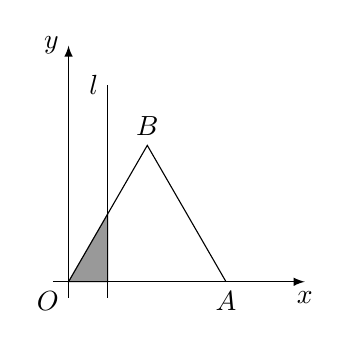
\begin{tikzpicture}[>=latex]
        \filldraw [gray!80] (0,0) -- (60:1) -- (0.5,0) -- cycle;
        \draw [->] (-0.2,0) -- (3,0) node [below] {$x$};
        \draw [->] (0,-0.2) -- (0,3) node [left] {$y$};
        \draw (0,0) -- (60:2) node [above] {$B$} -- (2,0) node [below] {$A$};
        \draw (0,0) node [below left] {$O$};
        \draw (0.5,-0.2) -- (0.5,2.5) node [left] {$l$};
    \end{tikzpicture}
\end{center}
\item 已知函数$f(x)=\sqrt {x+1}+\sqrt {1-x}$, 函数$g(x)=\sqrt {2-x}-\sqrt {1-x}$, 求函数$y=f(x)+g(x)$.
\item 已知函数$f(x)=\dfrac 1x$, 函数$g(x)=x^2-x$, 求函数$y=f(x)\cdot g(x)$.
\item 已知函数$f(x)=2x-\dfrac 1{x^2-1}$, 函数$g(x)=\dfrac 1{x^2-1}-1$.\\
(1) 求函数$y=f(x)+g(x)$;\\
(2) 画出函数$y=f(x)+g(x)$的图像.
\item 已知函数$f(x)=x\sqrt {x-1}$, 函数$g(x)=\sqrt {x-1}$, 设$F(x)=f(x)\cdot g(x)$.\\
(1) 写出$F(x)$的解析式;\\
(2) 画出$F(x)$的图像.
\item 已知函数$f(x)=x^2+x+1$, 求函数$y=g(x)$, 使$f(x)+g(x)=2x+4$.
\item 已知函数$f(x)=\dfrac{x^2+1}x$, 函数$g(x)=\dfrac{2x^2+1}x$, 函数$h(x)=x^2+1$, 求$F(x)=f(x)-g(x),H(x)=\dfrac{f(x)}{h(x)}$.
\item 已知函数$f(x)=\dfrac{x^2}{\sqrt {4-{x^2}}}$, 函数$g(x)=\sqrt {4-x^2}$.\\
(1) 求函数$y=f(x)\cdot g(x)$;\\
(2) 作出函数$F(x)=\begin{cases} f(x)\cdot g(x), & x\le 0, \\ x, & 0<x\le 2 \end{cases}$的图像.
\item 已知函数$f(x)=x^2,x\in (0,2)$, 函数$y=f(x)+g(x)$的图像如图所示, 写出函数$y=g(x)$的一个解析式.
\begin{center}
    \begin{tikzpicture}[>=latex]
        \draw [->] (-0.2,0) -- (2.5,0) node [below] {$x$};
        \draw [->] (0,-0.2) -- (0,2.5) node [left] {$y$};
        \draw (0,0) node [below left] {$O$};
        \draw (0,0) -- (2,2);
        \draw [dashed] (2,0) node [below] {$2$} -- (2,2) -- (0,2) node [left] {$2$};
        \filldraw [fill = white, draw = black] (0,0) circle (0.05) (2,2) circle (0.05);
    \end{tikzpicture}
\end{center}
*****
\item 选择题
若函数$y=f(x)$的定义域为R, 则$y=f(x)$为奇函数的充要条件为\bracket{20}.
\fourch{$f(0)=0$}{对任意$x\in \mathbf{R},f(x)=0$}{存在某个$x_0\in \mathbf{R}$, 使得$f(x_0)+f(-x_0)=0$}{对任意的$x\in \mathbf{R}$, $f(x)+f(-x)=0$都成立}
\item 求证下列函数为奇函数:
(1)$f(x)=x^{-3}$								(2)$f(x)=\dfrac x{1-x^2}$
\item 判断下列函数的奇偶性:
(1)$f(x)=2x+\sqrt[3]x$						(2)$f(x)=2x^1-x^2$
(3)$f(x)=x^2-x$							(4)$f(x)=\dfrac{1-x}{1+x}$
\item 已知函数$y=f(x)$的定义域为$[0,+\infty)$.如果对任意的$x>0$, 都有$f(x)<f(0)$, 那么函数$y=f(x)$有$[0,+\infty)$上是否一定是减函数?
\item 求证: 函数$f(x)=x-\dfrac 1x,x\in (-\infty ,0)$是增函数.
\item 判断函数$f(x)=2x+\dfrac 2x,x\in [\dfrac 12,3]$的单调性, 并求出它的单调区间.
\item 填空:
(1)如果函数$y=x^2-2mx+1$在$(-\infty ,2]$上是减函数, 那么实数m的取值范围是\blank{50}.
(2)当函数$f(x)=$				时, 函数$f(x)$同时满足条件: \textcircled{1} 函数$f(x)$不是偶函数; \textcircled{2} 在区间$(-\infty ,-1)$上是减函数; \textcircled{3} 在区间$(0,1)$上是增函数(写出一个你认为正确的函数解析式).
\item 求下列函数的最大值或最小值, 并求出取最值时相应的自变量x的值.
(1)$f(x)=x^2-4x-2$
(2)$f(x)=6x-3x^2$
(3)$f(x)=-x^2-4x-3,x\in [-3,1]$
(4)$f(x)=x^2-2x-3,x\in [-2,0]$
\item 已知p、q分别是函数$f(x)=-2x+3$在$[-2,2]$上的最大值和最小值, 求函数$g(x)=2x^2-px+q$在$[-2,2]$上的最大值和最小值.
\item 求函数$y=\dfrac 2{x-1}(2\le x\le 6)$的最大值与最小值.
\item 求函数$f(x)=x^3+x^2+x-1$在区间$(0,1)$内的零点(精确到0.1).
\item 画出函数$y=x^2-2|x|$的图像, 并写出它的定义域、奇偶性、单调区间、最小值.
\item 研究函数$f(x)=\dfrac 1{1+x^2}$的定义域、奇偶性、单调性、最大值.
习题3.4  B组
\item 已知函数$f(x)=|x-a|$, 且$f(1)=0$.
(1)求函数$y=f(x)$的解析式.
(2)比较$f(2)$与$f(-3)$的大小.
\item 已知函数$f(x)=x^2+ax+1,x\in [b,2]$是偶函数, 求a、b的值.
\item 已知函数$f(x)$为偶函数, $g(x)$为奇函数, 且$f(x)+g(x)=f(x)=x^2+2x+3$, 求$y=f(x)y=g(x)$的解析式.
\item 已知$a\ne 0$, 试讨论函数$f(x)=\dfrac a{1-x^2}$在区间$(0,1)$上的单调性.
\item 已知$\alpha \beta$是方程$\text4x^24mx+m+2=0$的两个实数根, 当m为何值时, $\alpha ^2+\beta ^2$有最小值? 并求出这个最小值.
\item 求函数$y=x^2-4x+1$在$x\in [t,4]$上的最小值和最大值, 其中$t<4$.
\item 已知集合$A=\{x|1\le x\le 4\},f(x)=x^2+px+q$和$g(x)=x+\dfrac 4x$是定义在A上的函数, 且在$x_0$处同时取到最小值, 并满足$f(x_0)=g(x_0)$, 求$f(x)$在A上的最大值.
\item 已知某气垫船的最大船速是48海里/时, 船每小时使用的燃料费用和船速的平方成正比, 若船速为30海里/时, 则船每小时的燃料费用为600元.其余费用(不论船速为多少)都是每小时864元.甲乙两地相距100海里, 船从甲地行驶到乙地.
(1)试把船每小时使用的燃料费用P(元)表示成船速v(海里/时)的函数.
(2)试把船从甲地到乙地所需的总费用y表示成船速v(海里/时)的函数.
(3)当船速为每小时多少海里时, 船从甲地到乙地所需的总费用最少?
\item 已知函数$y=f(x)$, 定义$F(x)=f(x+1)-f(x)$.某公司每月最多生产 100台报警系统装置, 生产x台$(x>0)$的收入函数为$R(x)=3000x-20x^2$(单位: 元), 其成本函数为$G(x)=5000x+4000$(单位: 元), 利润是收入与成本之差.
(1)求利润函数$y=f(x)$及相应的$y=F(x)$.
(2)利润函数$y=f(x)$与$y=F(x)$是否具有相等的最大值?
\item 求方程的近似解$x^2+2+\dfrac 1x=0$(精确到0.1).
\item 研究函数$f(x)=x+\dfrac ax(a>0)$的定义域、奇偶性、单调性.
复习题
A组
\item 求函数$y=\dfrac 1{2-x}+\sqrt {x^2-1}$的定义域.
\item 判断下列函数的奇偶性:
(1)$f(x)=|\dfrac 12x-3|+|\dfrac 12x+3|$				(2)$f(x)=x^3+\dfrac 2x$
(3)$f(x)=x^2,x\in (k,2)$
\item 已知$y=f(x)$是奇函数, 定义域为R, $y=g(x)$是偶函数, 定义域为D.设$F(x)=f(x)\cdot g(x)$, 判断$y=F(x)$奇偶性.
\item 已知函数$f(x)=(m-1)x^2+3x+(2-n)$, 且此函数为奇函数, 求m、n的值.
\item 已知函数$f(x)=x,g(x)=-\dfrac 4x,p(x)=f(x)-g(x)$, 求$y=p(x)$的函数表达式, 并写出$y=p(x)$的单调递减区间.
\item 分别作出下列函数的图像, 并指出它们的单调区间:
(1)$y=|x^2-4x|$							(2)$y=2|x|-3$
\item 设函数$f(x)=(a^2+4a-5)x^2-4(a-1)x+3$的图像都在x轴的上方, 求实数a的取值范围.
\item 已知函数$f(x)=x^2+10x-a+3$, 当$x\in [-2,+\infty)$时, $f(x)\ge 0$恒成立, 求实数a的取值范围.
\item 设$\alpha \beta$是二次方程$x^2-2kx+k+20=0$的两个实数根, 当k为何值时, $(\alpha +1)^2+(\beta +1)^2$有最小值?
\item 已知$f(x)=x^2+ax+1$, 若对任意的实数x, 均有$f(2+x)=f(2-x)$恒成立, 求实数a的值.
复习题
B组
\item 已知二次函数$f(x)=ax^2-2ax+3-a(a>0)$, 比较$f(-1)$和$f(2)$的大小.
\item 已知函数$f(x)=-x^2+2ax+1-a$在$[0,1]$上有最大值2, 求实数a的值.
\item 已知$y=f(x)$是定义在$(-1,1)$上的奇函数, 在区间$[0,1)$上是减函数, 且$f(1-a)+f(1-a^2)<0$, 求实数a的取值范围.
\item 已知函数$f(x)=2-x^2$, 函数$g(x)=x$, 定义函数$F(x)$如下: 当$f(x)\ge g(x)$时, $F(x)=g(x)$; 当$f(x)<g(x)$时, $F(x)=f(x)$.求$F(x)$的最大值.
\item 已知函数$y=f(x)$具有如下性质: (1)定义在R上的偶函数; (2)在$(-\infty ,0)$上为增函数; (3)$f(0)=1$; (4)$f(-2)=-7$; (5)不是二次函数.
求$y=f(x)$的一个可能的解析式.
\item 打开水龙头, 让水匀速地注入一个杯子内, 随着时间的增加, 杯中水面的高度不断增加, 直至水满溢出.在这个过程中, 杯中水面的高度h关于注水时间t的函数为$h=f(t)$.
(第6题)
(1)如果甲杯、乙杯的开头分别如图所示, 那么下列草图中, 甲杯相应函数$h=f(t)$的图像是\blank{50}, 乙杯相应函数$h=f(t)$的图像是\blank{50}.(只有杯子的圆柱和圆锥形部分可以盛水)
(第6(1)题)
(2)下列是两个杯子相应函数$h=f(t)$的图像, 试说明这两个杯子开头有何差别.
(第6(2)题)
第四章  幂函数、指数函数和对数函数(上)
\item 1  幂函数的图像与性质
习题4.1  A组
\item 已知幂函数$f(x)$的图像经过$(2,\dfrac{\sqrt 2}2)$, 试求出这个函数的解析式.
\item 填空:
幂函数$y=x^s$与$y=x^l$的图像在第一象限都通过定点\blank{50}, 若它们在第一象限的部分关于直线$y=x$对称, 则s、t就满足的条件是\blank{50}.
\item 研究幂函数$f(x)=x^{\dfrac 25}$的定义域、奇偶性、单调性、值域.
\item 作函数$y=\dfrac{|x|+1}{|x+1|}$的大致图像.
\item 已知函数$f(x)=x^3-3x$.
(1)试求函数$y=f(x)$的零点.
(2)求证: 函数$f(x)=x^3-3x$在$[1,+\infty)$上是增函数.
(3)是否存在自然数n, 使$f(n)=1000$? 若存在, 求出一个满足条件的n; 若不存在, 请问明理由.
习题4.1  B组
\item 在下列函数中, 哪一个既是奇函数, 又在区间$(+\infty ,0)$内是减函数?
(1)$y=x^{\dfrac 12}$; 		(2)$y=x^{\dfrac 13}$; 		(3)$y=x^{\dfrac 23}$; 		(4)$y=x^{-\dfrac 13}$.
\item 已知幂函数$f(x)$的定义域是$(+\infty ,0)\cup (0,+\infty)$, 且它的图像关于y轴对称, 写出一个满足要求的幂函数$f(x)$.
\item 已知函数$f(x)=\dfrac{ax+1}{x+2},a\in \mathbf{Z}$.是否存在整数a, 使函数$f(x)$在$x\in [-1,+\infty)$上递减, 并且$f(x)$不恒为负? 若存在, 找出一个满足条件的a; 若不存在, 请说出理由.
\item 2  指数函数的图像与性质
习题4.2  A组
\item 比较下列各题中两个值的大小:
(1)$3^{0.8},3^{0.7}$							(2)$0.75^{0.1},0.75^{-0.1}$
\item 设$a^{2x}=2$, 且$a>0,a\ne 0$, 求$\dfrac{{a^{3x}}+{a^{-3x}}}{{a^x}+{a^{-x}}}$的值.
\item 已知$f(x)=a\cdot b\cdot f(4)=648,f(5)=1944$.
(1)估算$f(4.5)$.
(2)计算$f(4.5)$, 利用计算的结果评判你的估算.
\item 已知$f(x)=3^x,uv\in \mathbf{R}$.
(1)求证: 对任意的u、v, 都有$f(u)\cdot f(v)=f(u+v)$成立.
(2)写出一个关于$f(u)\div f(v)$类似上式的等式, 并证明你的结论.
\item (1)求证: $f(x)=\dfrac{a^x-a^{-x}}2(a>0,a\ne 1)$是奇函数.
(2)求证: $f(x)=\dfrac{({a^x}-1)\cdot }{{a^x}+1}(a>0,a\ne 1)$是偶函数.
\item 选择题:
(1)若指数函数$y=a^x$是减函数, 则下列不等式中, 能够成立的是\bracket{20}.
\fourch{$a>1$}{$a<1$}{$a(a-1)<0$}{$a(a-1)>0$}
(2)若函数$y=2^x-m$的图像不经过第二象限, 则m的取值范围是\bracket{20}.
\fourch{$m\ge 1$}{$m<1$}{$m>-1$}{$m\le -1$}
\item 某地区的中小学2003年、2004年共购置电脑100台, 为了加快中小学的电脑普及程度, 准备新购置的电脑数按每两年递增10%的比例增长, 从2005年至2010年, 该地区中小学新购置的电脑总数是多少?
习题4.2  B组
\item 已知集合$M=\{y|y=2^x,x\in \mathbf{R}\}$, 集合$N=\{y|y=x^2,x\in \mathbf{R}\}$, 求$M\cap N$.
\item 作下列函数的大致图像:
(1)$y=2^{|x|}$							(2)$y=2^{-|x|}$
\item 判断并证明下列函数的奇偶性:
(1)$y=\dfrac{{{10}^x}-{{10}^{-x}}}{{{10}^x}+{{10}^{-x}}}$					(2)$y=x(\dfrac 1{2^x-1}+\dfrac 12)$.
\item 选择题:
函数$y=4^x-2^{x+1}+1(x<0)$的值域是
\fourch{$[0,+\infty)$}{$(1,+\infty)$}{$(0,1)$}{$(0,1]$}
复习题
A组
\item 幂函数$y=f(x)$, 当$x=2$时, $y=16$.
(1)求函数$f(x)$的解析式.
(2)比较$f(2)$和$f(-3)$的大小.
\item 填空:
(1)若关于x的方程$5^x=\dfrac{a+3}{5-a}$有负数根, 则a的取值范围是\blank{50}.
(2)方程$(\dfrac 12)^x=x^{\dfrac 12}$的实数根个数为\blank{50}.
\item 设在海拔x米处的大气压强是y帕, y与x之间的函数关系式是$y=c\cdot e^{k\tau }$, 其中c、k常量.已知某地某天在海平面的大气压强为$1.01\times 10^5$帕, 1 000米高空的大气压强为$0.90\times 10^5$帕, 求600米高空的大气压强.(结果保留3位有效数字)
\item 2005年1月6日, 我国人口总数为13亿, 称该天为``中国人口13亿日'', 如果2005年1月6日后我国人口的年自然增长率保持在0.6%, 问到哪一年我国人口总数将超过14亿?
\item 当x充分大时, 试比较下列各函数: $y_1=10x,y_2=8x^2,y_3=4x^4,y_4=2\times 3^x,y_5=5^x$值的大小.你能从中归纳出一些规律性的结论吗?
复习题
B组
\item 比较下列各题中两个值的大小(其中$a>0$, 且$a\ne 0$);
(1)$a^2$和$a^a$							(2)$2^a$和$a^a$
\item 把物体放在温度为$\theta _0$℃的空气中冷却, 若物体原来的温度是$\theta _0^\circ C(\theta _1>\theta _0)$, t分钟后物体温度$\theta _0$℃可由公式$\theta =\theta _0+(\theta _1-\theta _0)e^{-kt}$求得, 其中k是一个随着物体与空气的接触状况而定的常量, 现有62℃的物体, 放在15℃的空气中冷却1分钟以后物体的温度是52℃, 求上式中k的值(精确到0.01).开始冷却2分钟后物体的温度是多少? 开始冷却10分钟后, 物体的温度是多少? (精确到1℃).
总复习题
A组
\item 填空:
(1)若集合$A=\{y|y=x^2+2c+3\}$, 集合$B=\{y|y=x+\dfrac 4x\}$, 则$A\cup B$=		.
(2)已知$xy\in \mathbf{R}$, 集合$\alpha =\{(x,y)|xy\ge 0\}$, 集合$\beta =\{(x,y)||x+y|=|x|+|y|\}$, 用推出关系表示$\alpha \beta$的关系\blank{50}.
(3)若函数$f(x)=3x+1$的定义域为$\{1,3,k\}$.值域为$\{4,a^4,a^2+3a\}$, 且a、k为自然数, 则$a+k$=\blank{50}.
(4)已知函数$f(x)=\begin{cases} -2^r-1(x\le 0), \\ x^{\dfrac 12}(x>0). \end{cases}$若$f(x_0)=1$, 则$x_0$的值为\blank{50}.
(2)选择题:
(1)下列图形中, 能作为某个函数的图像的只能是						\bracket{20}.
(第2(1)题)
(2)若集合$A=\{x|0.1<\dfrac 1x<0.3,x\in \mathbf{N}\}$, 集合$B=\{x||x|\le 5,x\in \mathbf{Z}\}$, 则$A\cup B$中的元素个数是															\bracket{20}.
\fourch{11}{13}{15}{17}
(3)``$x\ne 1$且$y\ne 2$''是``$x+y\ne 3$''的								\bracket{20}.
\fourch{充分非必要条件}{必要非充分条件}{充要条件}{既非充分又非必要条件}
\item 点$(\sqrt 2,2)$在幂函数$y=f(x)$的图像上, 点$(-2,\dfrac 14)$在幂函数$y=g(x)$的图像上.当x为何值时, $f(x)=g(x)$?
\item 已知集合$A=\{x|3x^2+x-2\ge 0,x\in \mathbf{R}\}$, 集合$B=\{x|\dfrac{4x-3}{x-3}>0,x\in \mathbf{R}\}$, 求$A\cap B$.
\item 已知函数$f(x)=a^x(a>0,a\ne 1)$在区间$[1,2]$上的最大值比最小值大$\dfrac 14$, 求实数a的值.
\item 已知集合$A=(-2,-1)\cup (0,+\infty)$, 集合$B=\{x|x^2+ax+b\le 0\}$, 且$A\cap B=(0,2],A\cup B=(-2,+\infty)$, 求实数a、b的值.
\item 已知关于x的不等式$ax^2+3ax-2<0$的解集为R, 求实数a的取值范围.
\item 某地区某日海拔高度与气温的对照表为:
高度h(米)	0	500	1 000 	2 000
气温t(℃)	15.00	11.75	8.50	2.00
(1)根据表中t与h的对应关系, 写出t关于h的函数解析式.
(2)根据(1)的结论, 求海拔高度1 500米处的气温.
\item (1)指出函数$f(x)=ax^2+\dfrac b{x^2}$(a、b是正常数)所具有的基本性质, 并加以说明.
(2)当$a=\dfrac 14,b=4$时, 画出函数$f(x)=ax^2+\dfrac b{x^2}$的简图.
\item 若$2x+y=1$, 求$4^x+2^y$的最小值.
总复习
B组
\item 已知集合$A=\{x||x-a|<2\}$, 集合$B=\{x|\dfrac{2x-1}{x-2}<1\}$, 且$A\subseteq B$, 求实数a的取值范围.
\item 已知全集$U=\mathbf{R}$, 集合$A=\{x|x^2+px+12=0\}$, 集合$B=\{x|x-5x-q=0\}$, 满足$(\complement _UA)\cap B=\{2\}$.求实数p与q的值.
\item 试讨论函数$f(x)=\dfrac x{1-x^2}$在区间$(-1,1)$上的单调性.
\item 甲乙两地的高速公路全长166千米, 在高速公路上最高行驶时速不得高于120千米/时, 假设汽车从甲地进入该高速公路以不低于70千米/时的速度匀速行驶到乙地, 已知汽车每小时的运输成本(以元为单位)由可变部分和固定部分组成: 可变部分与速度v(千米/时)的平方成正比, 比例系数为0.02; 固定部分为220元.
(1)把全程运输成本y(元)表示为速度v(千米/时)的函数, 并指出这个函数的定义域.
(2)汽车应以多大速度行驶才能使全程运输成本最小? 最小运输成本约为多少元?
\item 某居民小区供水站的蓄水池现有水40吨, 自来水厂每小时可向蓄水池中注水8吨, 同时蓄水池又向居民小区供水, t小时内供水总量为$32\sqrt t$吨.现在开始向池中注水并同时向居民小区供水, 若蓄水池中存水量少于10吨, 就会出现供水紧张现象.
(1)试建立蓄水池中存水量S与供水时间t之间的函数关系.
(2)供水多少时间开始出现供水紧张? 这一天内供水紧张的有几小时?
.
第四章  幂函数、指数函数和对数函数(下)
\item 4  对数概念及其运算
习题4.4  A组
\item 把下列指数式写成对数式:
(1)$10^{-2}=0.01$.						(2)$(\dfrac 12)^0=1$.
(3)$5^x=6$.
\item 把下列对数式写成指数式:
(1)$x=\log _{16}32$.					(2)$\log _{\pi }x=4$.
(3)$\log _x9=2$.
\item 求下列各式中的$x$:
(1)$\log _{\dfrac 12}x=3$.						(2)$\log _3\dfrac 1{27}=x$.
(3)$\log _{100}1000=x$.					(4)$\log _x16=4$.
\item 计算:
(1)$\log _55\sqrt 5+\ln e$.					(2)$\lg \sqrt {10}-\lg 0.01$.
(3)$\log _{12}6+\log _{12}2$					(4)$\log _348-4\log _32$.
\item 用$\log _aM$、$\log _aN$表示下列各式:
(1)$\log _aMN^2$.						(2)$\log _a\dfrac{\sqrt M}N$.
\item 计算:
(1)$3^{\log _31}+\log _248-\log _23$.
(2)$2\log _7\dfrac{35}9+4\log _73+2\log _7\dfrac 1{10}+\log _74$.
\item 计算:
(1)$\log _32\times \log _53\times \log _85$.			(2)$(\log _43+\log _83)\times \log _32$.
(3)$\log _2\dfrac 1{49}\times \log _3\dfrac 1{16}\times \log _7\dfrac 1{27}$.		(4)$\log _ab\cdot \log _bc\cdot \log _ca$.
(5)$(\log _43+\log _83)(\log _32+\log _94)$.
\item 已知$\log _32=m$, 试用$m$表示$\log _{32}18$.
\item 已知$\lg 2=a$, $\lg 3=b$.
(1)求$\lg 5$.
(2)求$\log _23$.
(3)求$\log _{12}25$.
习题4.4  B组
\item 求出下列各式中$x$的取值范围: ($a>0$且$a\ne 1$)
(1)$\log _a(x^2+1)$.					(2)$\log _a(x-2)$.
(3)$\log _a\dfrac 1{x+2}$.
\item 在下列各式中的括号内填入适当的值, 使等式成立:
(1)$\log _5()=1$	.					(2)$2^{\log _31}=()$.
(3)$(\dfrac 15)^{\log _{0.2}3}=()$.					(4)$\sqrt 3^{\log _{\sqrt 3}()}=7$.
\item 用$\log _ax$、$\log _ay$、$\log _a(x+y)$、$\log _a(x-y)$表示下列各式:
(1)$\log _a(x^2-y^2)$.					(2)$\log _4\dfrac{{x^3}y}{{{(x+y)}^4}}$.
(3)$\log _a(\dfrac{\sqrt x}{\sqrt y}-\dfrac{\sqrt y}{\sqrt x})$.
\item 计算:
(1)$\log _2(\log _216)$.					(2)$2^{\log _65}\times 3^{\log _65}$.
(3)$\sqrt {1g^25-2\lg 5+1}$.				(4)$\lg ^25+\lg ^2\times \lg 50$.
\item 设$56^a=14$, 试用$a$表示$\log _756$.
\item 已知$5.4^x=3$, $0.6^y=3$, 求$\dfrac 1x-\dfrac 1y$的值.
\item 5  反函数的概念
习题4.5  A组
\item 已知函数$f(x)=x^2-4x-5$, $x\in [1,3]$, 判断其是否存在反函数.若存在, 求出反函数; 若不存在, 说明理由.
\item 求下列函数的反函数:
(1)$y=-x^3$.						(2)$y-\dfrac x{x+2}$.
(3)$y=x^2+1(x<0)$.
\item 已知$f(x)=1-x^2(x<-1)$, 求$f^{-1}(-3)$的值.
\item 已知函数$y=\dfrac a{x+1}$的反函数的图像经过点$(\dfrac 12,1)$, 求实数$a$的值.
\item 已知函数$y=f(x)$的图像与函数$y=\dfrac{x-1}{x+1}$的图像关于直线$y=x$对称, 求函数$y=f(x)$的解析式.
习题4.5  B组
\item 判断题: (正确的在括号内用``√''表示, 错误的用``×''表示)
(1)存在反函数的函数一定是单调函数.				\bracket{20}.
(2)偶函数存在反函数.							\bracket{20}.
(3)奇函数必存在反函数.							\bracket{20}.
\item 一次函数$y=-x$的图像与它的反函数的图像重合.试写出一个非一次函数的函数, 使它的图像与其反函数的图像重合.
\item 如果函数$y=f(x)$的图像过点$(0, 1)$, 那么函数$y=f^{-1}(x)+2$的反函数的图像过点\bracket{20}.
\fourch{(3, 0)}{(0, 3)}{(1, 2)}{(2, 1)}
\item 如果$y=-\sqrt {1-x^2}$的反函数是$y=-\sqrt {1-x^2}$, 那么原来的函数的定义域是\bracket{20}.
\fourch{$(0,+\infty)$;}{$[-1,1]$;}{$[-1,0]$;}{$[0,1]$}
\item 求函数$y=\begin{cases} -\sqrt x(0\le x\le 1), \\ x^2(-1\le x<0) \end{cases}$的反函数.
\item 6  对数函数的图像与性质
习题4.6  A组
\item 求下列函数的定义域:
(1)$y=\lg (x^2-3x+2)$.				(2)$y=\dfrac{\sqrt {2x-1}}{\lg x}$.
(3)$y=\sqrt {\lg x}+\lg (5-2x)$.
\item 求下列函数的反函数:
(1)$y=10^x+1$.						(2)$y=\log _2(x+1)$.
(3)$y=\log _22x$.
\item 已知函数$f(x)=a^x+b$的图像经过点(1, 7), 反函数$f^{-1}(x)$的图像经过点(4, 0), 求函数$f(x)$的表达式.
\item 根据下列不等式, 确定底数$a$的取值范围:
(1)$\log _40.2<\log _a0.1$.				(2)$\log _a\pi >\log _ae$.
(3)$\log _a3<0$.
\item 已知$1<x<2$, $a=2^x$, $b=\log _{0.5}x$, $c=\sqrt x$, 比较$a$、$b$、$c$的大小, 并说明理由.
\item 声音强度$D$(分贝)由公式$D=10\lg (\dfrac I{10^{-16}})$给出, 其中$I(W/cm^2)$为声音能量.能量小于$10^{-16}W/cm^2$时, 人听不见声音.能量大于60分贝属于噪音, 其中70分贝开始损害听力神经, 90分贝以上就会使听力受损, 而一般的人呆在100分贝-120分贝的空间内, 一分钟就会暂时性失聪.
(1)求人低声说话$I=10^{-13}W/cm^2$的声音强度.
(2)求噪音的能量范围.
(3)当能量达到多少时, 人会暂时性失聪?
习题4.6  B组
\item 判断函数$y=1g\dfrac{x+1}{x-1}$的奇偶性.
\item 设$a>0$且$a\ne 1$, 比较$\log _a2a$与$\log _a3a$的大小.
\item 求证: $y=1g(1-x)$在定义域上单调递减.
\item 求函数$y=\log _{\dfrac 15}(x^2-6x+10)$在区间$[1,2]$上的最大值.
\item 7  简单的指数方程
习题4.7  A组
\item 解下列方程:
(1)$2^{1-x}=\dfrac 1{32}$.						(2)$3^{-x+2}=9^x$.
(3)$4^{2x-1}=1$.						(4)$0.38\cdot 10^{x-3}=0.5$(精确到0.01).
\item 解下列指数方程:
(1)$2^{x^2+3}=(\dfrac 14)^{\dfrac 22}$.					(2)$9^x-8\cdot 3^x-9=0$.
\item 已知关于$x$的方程$2a^{2x-2}-7a^{x-1}+3=0$有一个根是$x=2$, 求$a$的值并求方程的其余的根.
\item 某种放射性物质不断衰减, 若每经过一年剩留的物质是原来的$\dfrac 45$, 经过多少年, 剩流物质是原来的$\dfrac{64}{125}$?
习题4.7  B组
\item 解方程: $9^x+4^x=\dfrac 52\cdot 6^x$.
\item 解方程: $4^x+4^{-x}-6(2^x+2^{-x})+10=0$.
\item 动物尸体内$^{14}C$的含量每年衰减$0.12$, 设动物死亡的时刻$t=0$时, $^{14}C$含量为$100\%$.
(1)写出$^{14}C$含量$y$关于时间$t$的函数解析式.
(2)$^{14}C$含量减少到$50\%$需多少时间? (精确到1年)
\item 8  简单的对数方程
习题4.8  A组
\item 解下列方程:
(1)$\log _3(x-2)=1$.					(2)$\log _2(x^2-3x)=2$.
(3)$\log _2(\log _5x)=1$.				(4)$\log _5(x+1)-\log _{\dfrac 15}(x-3)=1$.
\item 解下列方程:
(1)$\log _2^2x+3\log _2x+2=0$.			(2)$\log _x(x^2-x)=\log _x2$.
\item 解下列方程:
(1)$\log _{\dfrac 12}(9^{x-1}-5)=\log _{\dfrac 12}(3^{x-1}-2)-2$.	(2)$(\lg x)^2-\lg x^2=3$.
习题4.8  B组
\item 解方程: $x^{\log _2x}=32x^4$.
\item 求方程$\log _2(x+4)=(\dfrac 13)^x$根的个数, 并说明理由.
复习题
A组
\item 填空:
(1)若$x^5=3$, 则$x=$\blank{50}; 若$5^x=3$, 则$x=$\blank{50}.
(2)计算: $\log _236-2\log _23=$\blank{50}.
(3)若$\log _ab\cdot \log _5a=3$, 则$b=$\blank{50}.
(4)函数$y=\log _2x(x\ge 1)$的反函数是\blank{50}.
(5)若点(1, 7)既在函数$y=\sqrt {ax+b}$的图像上, 又在其反函数的图像上, 则数对$(a,b)$为
\blank{50}.
\item 选择题:
(1)若$f(x)=3^x+5$, 则$f^{-1}(x)$的定义域是\bracket{20}.
\fourch{$(0,+\infty)$;}{$(5,+\infty)$;}{$(8,+\infty)$;}{$(-\infty ,+\infty)$}
(2)若$\log _{18}9=a$, $18^b=5$, 则$\log _{36}45$等于\bracket{20}.
\fourch{$\dfrac{a+b}{2+a}$;}{$\dfrac{a+b}{2-a}$;}{$\dfrac{a+b}{2a}$;}{$\dfrac{a+b}{a^2}$}
\item 已知函数$f(x)=\dfrac{ax+1}{x-3}$的反函数是$f(x)$本身, 求实数$a$的值.
\item 作出下列函数的图像:
(1)$y=\log _2(x-1)$.					(2)$y=|\log _2(x-1)|$.
\item 已知$\lg x+\lg y=2$, 求$\dfrac 1x+\dfrac 1y$的最小值.
\item 解下列方程:
(1)$4^x+2^{x+1}=80$.					(2)$\lg (2x+2)+\lg (15-x)=1+\lg 3$.
\item 已知函数$f(x)=\log _a\dfrac{1+x}{1-x}(a>0,a\ne 1)$.
(1)求$f(x)$的定义域.
(2)判断$f(x)$的奇偶性, 并加以证明.
(3)当$a>1$时, 求使$f(x)>0$的$x$的取值范围.
\item 如果光线每通过一块玻璃其强度要减少$10\%$, 求至少需要多少块这样的玻璃重叠起来, 才能使通过它们的光线强度为原来的强度的$\dfrac 13$以下?
复习题
B组
\item 填空:
(1)如果函数$f(x)=\log _a(-x^2+ax)$的定义域为$(0,\dfrac 12)$, 那么实数$a=$\blank{50}.
(2)如果$45^x=3$, $45^y=5$, 那么$2x+y=$\blank{50}.
(3)若函数$y=f(x)$的图像与函数$y=2^x-1$的图像关于直线$y=x$成轴对称图形, 则函数$y=f(x)$的解析式为\blank{50}.
\item 选择题:
(1)当$a>1$时, 在同一坐标系中, 函数$y=a^{-x}$与$y=\log _ax$的图像是\bracket{20}.
(2)函数$f(x)=4+\log _a(x-1)(a>0a\ne 1)$的图像恒经过定点$P$, 则点$P$的坐标是\bracket{20}.
\fourch{(1, 4);}{(4, 1);}{(2, 4);}{(4, 2)}
\item 已知$0<a<1$, 化简$\sqrt {\lg ^2a-\lg \dfrac{a^2}{10}}$.
\item 已知$\alpha$、$\beta$是方程$\lg ^2x-\lg x-2=0$的两根, 求$\log _{\alpha }\beta +\log _{\beta }\alpha$的值.
\item 判断命题``若函数$y=f(x)$与$y=f^{-1}(x)$的图像有公共点, 则公共点必在直线$y=x$上''的真假, 并说明理由.
\item 如果$^{237}U$在不断的裂变中, 每天所剩留质量与上一天剩留质量相比, 按同一比例减少, 经过7天裂变, 剩留的质量是原来的$50\%$, 计算它经过多少天裂变, 剩留质量是原来的$10\%$.


\end{enumerate}
\end{document}